
\documentclass[tikz,border=3pt]{standalone}
\usetikzlibrary{arrows.meta,positioning}
\begin{document}
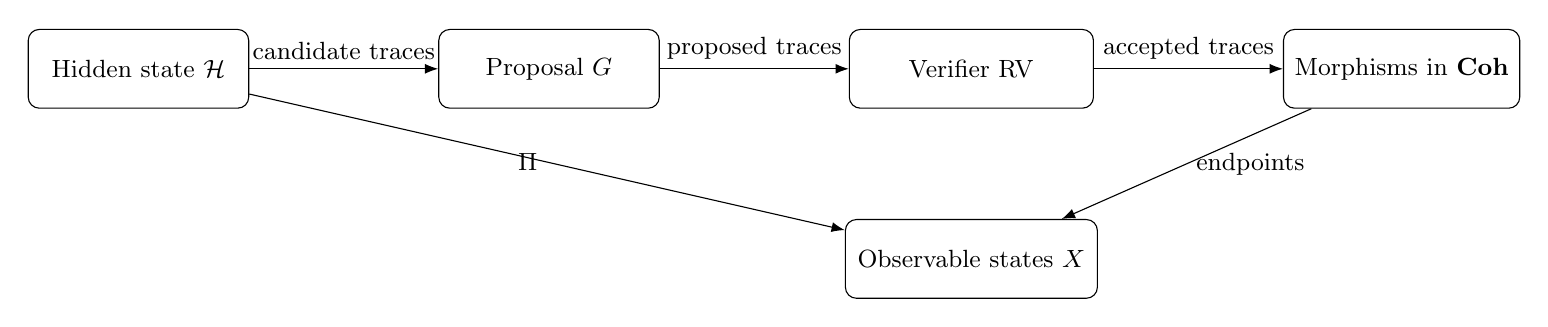
\begin{tikzpicture}[node distance=2.4cm, every node/.style={font=\small}]
\node[draw, rounded corners, minimum width=2.8cm, minimum height=1cm] (hid) {Hidden state $\mathcal H$};
\node[draw, rounded corners, minimum width=2.8cm, minimum height=1cm, right=of hid] (gen) {Proposal $G$};
\node[draw, rounded corners, minimum width=3.1cm, minimum height=1cm, right=of gen] (ver) {Verifier $\mathrm{RV}$};
\node[draw, rounded corners, minimum width=3cm, minimum height=1cm, right=of ver] (cat) {Morphisms in $\mathbf{Coh}$};
\node[draw, rounded corners, minimum width=3.2cm, minimum height=1cm, below=1.4cm of ver] (obs) {Observable states $X$};

\draw[-{Latex}] (hid) -- node[above] {candidate traces} (gen);
\draw[-{Latex}] (gen) -- node[above] {proposed traces} (ver);
\draw[-{Latex}] (ver) -- node[above] {accepted traces} (cat);
\draw[-{Latex}] (hid) -- node[left] {$\Pi$} (obs);
\draw[-{Latex}] (cat) -- node[right] {endpoints} (obs);
\end{tikzpicture}
\end{document}
